\section{Auswertung}
\label{sec:Auswertung}

\subsection{Bestimmung der Zerfallskurve und der Halbwertszeit von Indium}
Die Messdaten zur Bestimmung der Zerfallskurve und Halbwertszeit von Indium sind in Tabelle
\ref{tab:indium} aufgetragen.
Die Messzeit beträgt jeweils $\Delta t = \SI{240}{\second}$.
Weiterhin entspricht die Nullmessung $220$ Impulsen bei einer Messzeit von $\SI{900}{\second}$.
Damit werden immer -- durch die Übertragung auf die Messzeit $\Delta t = \SI{240}{\second}$ --
$\frac{176}{3}$ Zerfälle abgezogen.
\begin{table}
	\centering
	\caption{Messdaten der Zerfälle $N$ beim Zeitpunkt $t$ zur Bestimmung der Zerfallskurve und Halbwertszeit von Indium.}
	\label{tab:indium}
	\begin{tabular}{cc}
		\toprule
		$t$ / $\si{\second}$ & $N$ \\
		\midrule
		240 & 2576 \\
		480 & 2250 \\
		720 & 2116 \\
		960 & 1984 \\
		1200 & 1905 \\
		1440 & 1753 \\
		1680 & 1701 \\
		1920 & 1688 \\
		2160 & 1542 \\
		2400 & 1456 \\
		2640 & 1438 \\
		2880 & 1348 \\
		3120 & 1291 \\
		3360 & 1262 \\
		3600 & 1128 \\
		\bottomrule
	\end{tabular}
\end{table}
Gemäß Formel \eqref{eqn:halbwertszeit} wird die Anzahl der Zerfälle logarithmiert gegen die
Zeit aufgetragen.
Also ergibt sich der Zusammenhang
\begin{equation}
	\label{eqn:Halbwertszeit2}
	\ln N(t) = \ln N_0 - \lambda t \mathrm{.}
\end{equation}
Eine lineare Ausgleichsrechnung der Form
\begin{equation*}
	f(x) = m \cdot x + b
\end{equation*}
mit den Datentupeln $\{ t, \ln (N)\}$ aus Tabelle \ref{tab:indium} ergibt die Geradenparameter
\begin{align*}
	m &= (-\num{2,2(8)}) \cdot 10^{-4} \si{\per\second}  \, \mathrm{,} \\
	b &= \num{7,80(2)} \, \mathrm{.}
\end{align*}
Damit ist die Zerfallskonstante
\begin{equation*}
	\lambda = (\num{2,2(8)}) \cdot 10^{-4} \si{\per\second}  \, \mathrm{.} \\
\end{equation*}
Die zugehörige Ausgleichsgerade ist in Abbildung \ref{fig:indium} dargestellt.
Mit Formel \eqref{eqn:???} ergibt sich die Halbwertszeit von Indium $^{116}\mathrm{In}$
zu
\begin{equation*}
	\tau =  (\num{3.08(11)}) \cdot 10^3 \si{\second} \, \mathrm{.}
\end{equation*}
\begin{figure}
	\centering
	\includegraphics{Messdaten/indium.pdf}
	\caption{Messdaten der logarithmierten Zerfälle $N$ aufgetragen gegen die Zeit $t$ mit zugehöriger Ausgleichgerade gemäß Formel \eqref{eqn:halbwertszeit} bzw. Formel \eqref{eqn:Halbwertszeit2}.}
	\label{fig:indium}
\end{figure}






\subsection{Untersuchung der Halbwertszeit der beiden Zerfälle bei Silber}
Die Nullmessung bluzp


Zweiter Prozess
m -0.0061+/-0.0013
b 3.3+/-0.4
Halbwertszeit langer Zerfall 112.919500511

Erster Prozess
m  -0.0278+/-0.0018
b 5.11+/-0.11
Halbwertszeit kurzer Zerfall 24.9737013494


\begin{table}
\begin{tabular}{cccc}
t & n & n-nlang & ln(n) \\
8.0 & 136.0 & 122.6 & 4.81 \\
16.0 & 113.0 & 99.62 & 4.6 \\
24.0 & 91.0 & 77.65 & 4.35 \\
32.0 & 84.0 & 70.68 & 4.26 \\
40.0 & 62.0 & 48.71 & 3.89 \\
48.0 & 75.0 & 61.73 & 4.12 \\
56.0 & 51.0 & 37.76 & 3.63 \\
64.0 & 45.0 & 31.79 & 3.46 \\
72.0 & 37.0 & 23.82 & 3.17 \\
80.0 & 27.0 & 13.85 & 2.63 \\
88.0 & 33.0 & 19.87 & 2.99 \\
96.0 & 23.0 & 9.9 & 2.29 \\
104.0 & 21.0 & 7.93 & 2.07 \\
\end{tabular}
\end{table}


\begin{table}
	\centering
	\caption{Messwerte zur Bestimmung der Halbwertszeit des langlebigen Zerfalls für Silber.}
	\label{tab:silver2}
\begin{tabular}{ccc}
	\toprule
$t$/$\si{\second}$ & Anzahl der Zerfälle $N_\mathrm{l}$ & Logarithmus $\ln{N_\mathrm{l}}$ \\
\midrule
168.0 & 5.0 & 1.618 \\
176.0 & 8.0 & 2.085 \\
184.0 & 13.0 & 2.568 \\
192.0 & 6.0 & 1.799 \\
200.0 & 12.0 & 2.489 \\
208.0 & 5.0 & 1.618 \\
216.0 & 8.0 & 2.085 \\
224.0 & 10.0 & 2.307 \\
232.0 & 5.0 & 1.618 \\
240.0 & 8.0 & 2.085 \\
248.0 & 4.0 & 1.397 \\
256.0 & 6.0 & 1.799 \\
264.0 & 2.0 & 0.715 \\
272.0 & 10.0 & 2.307 \\
280.0 & 8.0 & 2.085 \\
288.0 & 6.0 & 1.799 \\
296.0 & 4.0 & 1.397 \\
304.0 & 7.0 & 1.952 \\
312.0 & 6.0 & 1.799 \\
320.0 & 1.0 & 0.043 \\
328.0 & 2.0 & 0.715 \\
336.0 & 6.0 & 1.799 \\
344.0 & 2.0 & 0.715 \\
352.0 & 6.0 & 1.799 \\
360.0 & 3.0 & 1.113 \\
368.0 & 2.0 & 0.715 \\
376.0 & 6.0 & 1.799 \\
384.0 & 1.0 & 0.043 \\
392.0 & 3.0 & 1.113 \\
400.0 & 1.0 & 0.043 \\
408.0 & 2.0 & 0.715 \\
416.0 & 3.0 & 1.113 \\
\bottomrule
\end{tabular}
\end{table}

\begin{figure}
  \centering
  \includegraphics{Messdaten/silber.pdf}
  \caption{Zerfallskurve für Silber samt beider Ausgleichgraden zur Bestimmung der verschieden ablaufenden Einzelzerfälle.}
  \label{fig:silber}
\end{figure}

\begin{figure}
  \centering
  \includegraphics{Messdaten/ergebnis.pdf}
  \caption{Darstellung des mittels Ausgleichsrechnungen ermittelten summierten Zerfalls sowie der im Experiment gemessenen Werte.}
  \label{fig:ergebnis}
\end{figure}


%Bild
%\begin{figure}
%  \centering
%  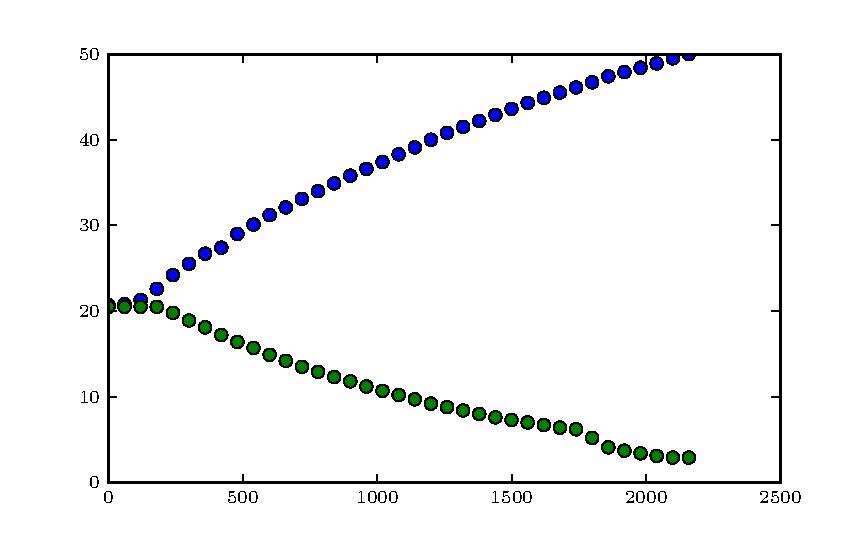
\includegraphics{plot.pdf}
%  \caption{Plot.}
%  \label{fig:plot}
%\end{figure}


%Tabelle
%\begin{table}
%	\centering
%	\caption{Table.}
%	\label{tab:table}
%	\begin{tabular}{ccc}
%		\toprule
%    column1&column2&column3\\
%		\midrule
%		220 & -391 & 659 \\
%		330 & -598 & 946 \\
%		525 & -1000 & 1660 \\
%		702 & -1337 & 2051 \\
%		930 & -1650 & 2450 \\
%		\bottomrule
%	\end{tabular}
%\end{table}
